% !TeX root = main.tex
\chapter{Software implementation}\label{app:tech}

As part of the research presented in this thesis, we developed several systems for semantic speech editing and audio
visualization. We have since published these systems as open-source software for others to use. This chapter outlines
the technical details behind the implementation of these systems, including notes on how we approached the more
challenging technical aspects of system design.

\section{Dialogger}\label{sec:dialogger}

\textit{Dialogger} is a semantic audio and video editor that enables the navigation and editing of media recordings using a
text-based interface. The design and operation of Dialogger is outlined in Section~\ref{sec:paper-screen-design}. We
have published the system as open-source software under an Apache 2.0 licence at the following URL:
\url{https://github.com/bbc/dialogger}

%Requirements:
%Correction (i.e. text editing)
%while retaining timestamps
%Editing (i.e. audio editing)
%Live preview of edits
%Display/edit speaker segments
%Display timestamps
%Export EDL

%Solution:
%Use CKEditor for text editing with restricted functionality
  %No cut/copy/paste or dragging
  %Replace only
  %Selections jump to start/end of words
  %Generate new timestamps when replacing >1 word
%Edit audio using bold/underline
%Use HTML5-video-compositor for preview
%JSON->HTML, HTML->JSON
%JSON->EDL

Dialogger includes features for playback, navigation and editing of media using a transcript, export of edit
decision lists (EDLs), user accounts and media asset management. Our system does not include an ASR system, media
transcoder or media file export, however these can easily be integrated using the instructions in the user guide.

\subsection{System overview}

The structure and data flow of Dialogger is shown in Figure~\ref{fig:dialogger-flow}. We divided our system into a
presentation layer (front end) and a data management layer (back end). The front end used HTML, CSS and Javascript so
that the system could be accessed through a web browser.  We used \textit{Semantic UI} as a user interface framework,
\textit{Backbone} as a model-view-controller framework and \textit{Dropzone} to handle file uploads.

\begin{figure}[t]
\centering
  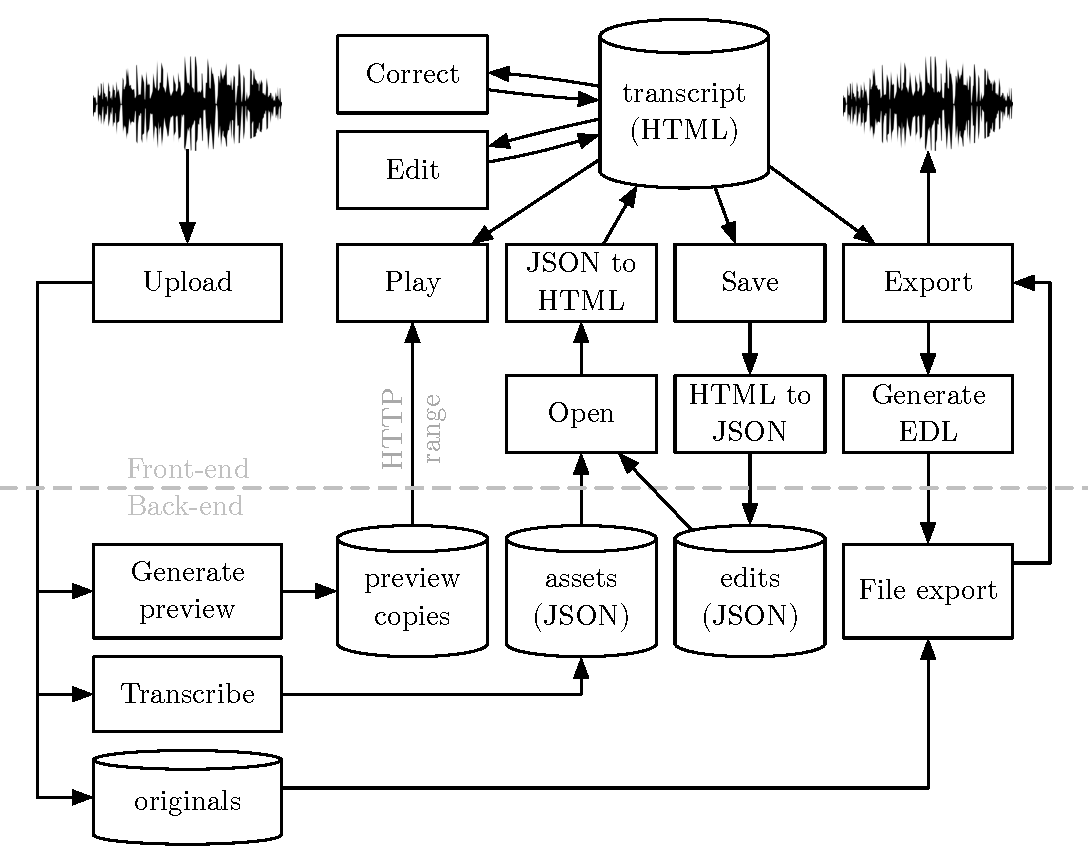
\includegraphics[width=.8\textwidth]{figs/dialogger-flow-diagram.pdf}
  \caption{Flow diagram of the Dialogger system. Excluded components are shaded.}
  \label{fig:dialogger-flow}
\end{figure}

For the back end, we used \textit{Node.js} and \textit{Express} as our framework, and \textit{MongoDB} for our
database. We authenticated users using \textit{Passport.js}, logged errors using \textit{Bunyan} and used
\textit{Mimovie} to extract metadata from uploaded media files.

\subsection{Word processing}

We included word processing functionality in Dialogger to allow users to navigate the speech, correct mistakes in the
transcript and mark up edit decisions.  We used the \textit{CKEditor}\footnote{\url{https://ckeditor.com/}} 
library as the basis for the word processing functionality in our interface.

\paragraph{Timestamps}
In addition to the requirements of a normal word processor, our system had a unique requirement for each word to
include a hidden timestamp, and for that timestamp to be retained throughout the editing process.  We achieved this by
using HTML formatting to add a tag to each word, and including the start and end timestamps as attributes of the 
tag. This linked the words to timestamps, but certain edit actions created problems, as explained below.

\paragraph{Split words}
Traditional word processors allow users to select text with the granularity of individual characters. This caused an
issue where words could be split by cutting, moving or replacing only part of a word. To avoid this problem, we
restricted editing to word level-granularity by automatically moving the user's selections to the start and end of
words.

\paragraph{Joined words}
Occasionally, ASR systems will transcribe a single word as two or more words. When the user corrects this by selecting
both words and typing a replacement, then both words are replaced and their timestamps are lost. To avoid this, we
added logic that detected this behaviour and created a new word with the start time of the first selected word and the end time
of the last selected word.

\paragraph{Re-ordering}
Word processing gives users the freedom to move and edit words as they wish.  However, when text is moved around it becomes
very difficult for the user to keep track of the original location and order of the words. This is a problem with audio
editing as some edits sound unacceptable, so users will often want to adjust the edit.
Our solution was to retain the sequence of the words so that they stay in their original positions. This prevented
re-ordering of the words, however, this could later be adjusted using a DAW.  We implemented this restriction by disabling cut,
copy, paste and drag-and-drop.

\subsection{Media integration}

We used timestamps to link each word in the transcript to a segment of a media file.  To integrate the transcript edits
with the media, we built systems to generate an edit decisions list (EDL) based on the user's annotations, to instantly
preview those edits in the browser, and to allow the user to download a copy of the final edit.

\paragraph{EDL generation}
In addition to including the start and end timestamp of each word in a HTML tag, we included the timestamp of the next
word in the transcript. To detect edit points, we simply looked for any difference in the predicted and actual timestamp
of the next word.  We could then generate an EDL by filtering words based on their annotation, then looking for edit points.
However, this approach relies on the words being in their original sequence.  Our EDL format is simply an array of
timestamps that denote the in-points and out-points of each edit.

\paragraph{Preview}
We wanted users to be able to preview their edits to quickly hear whether the edits sound acceptable or not.  When a
user uploads their media, we transcode a low-bitrate ``preview copy'' of the file, which we then use for live playback
in the browser.  To control the playback, we used \textit{HTML5 Video
Compositor}\footnote{\url{https://github.com/bbc/html5-video-compositor}} --- a media composition engine that can play
edit decision lists in the browser.  After the user makes an edit, we generate an EDL, convert it to the correct
format, and pass it to the compositor, which dynamically adjusts the playback of the preview copy.  To avoid the browser
having to download the entire file before playback, we used byte serving to dynamically send only the portion of the
preview copy that is needed.

\paragraph{Export}
Once the user has completed their production, they can export their edit as either a rendered media file, or an EDL
file for a DAW. The EDL of the user's edits is sent from the browser to the back end. Media is
rendered and transcoded using the \textit{MLT Multimedia Framework}\footnote{\url{https://www.mltframework.org/}} that
supports sample-accurate editing of audio and video files. To maximise the quality of the exported media, we use the original assets
when rendering the file. To generate the EDL files for DAWs, we simply convert our internal EDL format into
\citet{AES2008} or another proprietary format.

\clearpage
\section{Vampeyer}\label{sec:vampeyer}
As part of this research, we wanted to generate audio visualizations based on extracted semantic audio features.  There
are already many software packages that visualize audio, and audio features, in a variety of ways, most notably Sonic
Visualiser \citep{Cannam2010}.  However, the visualization algorithms are hard-coded into the software, making
prototyping of new methods difficult.  We developed a software plugin system for visualizing audio as a bitmap image.
We have published this system as open-source software under an Apache 2.0 licence at the following URL:
\url{https://github.com/bbc/dialogger}

\subsection{Design}
We built our plugin system on top of the well-known \textit{Vamp} audio analysis plugin
system\footnote{\url{http://vamp-plugins.org/}}, to make use of the current large collection of audio feature
extraction plugins.  An outline of the design of Vampeyer is shown in Figure~\ref{fig:vampeyer}.  We designed our
plugin system to receive the output of one or more Vamp plugins as the input, and send a bitmap image as the output.

\begin{figure}[ht]
  \centering
  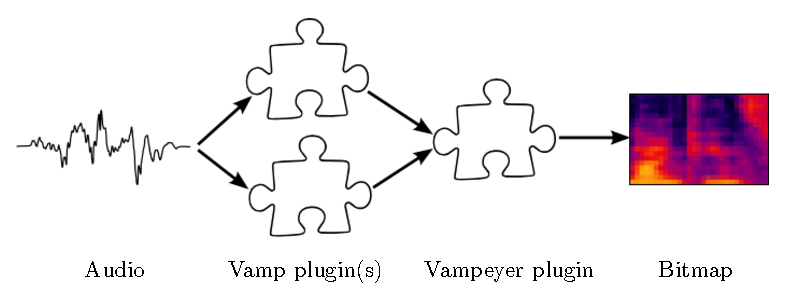
\includegraphics[width=0.8\textwidth]{figs/vampeyer.pdf}
  \caption{High-level system diagram of the Vampeyer visualization framework}
  \label{fig:vampeyer}
\end{figure}

A Vampeyer plugin defines which Vamp plugin(s) it requires, including the block/step size and parameters.  At least one
Vamp plugin is required, but there is no restriction of the number of Vamp plugins that can be used.  Both
frameworks are written in C++ which allows for efficient processing.  This is important when processing large
collections, or generating visualizations ``on-the-fly''.  Vampeyer plugins are compiled into shared libraries, so they can
be distributed without users having to re-compile locally and be integrated into third-party software.

\subsection{Implementation}
To illustrate the design and operation of Vampeyer plugins, we describe the data structures and functions that are used
to convert the Vamp plugin output into an image.  The following five data structures define how data should be sent and
returned from the plugin's functions.

{\singlespacing
\begin{itemize}
  \item \texttt{VampParameter} is a name/value pair used to store a parameter
  \item \texttt{VampParameterList} is a vector of \texttt{VampParameter}s
  \item \texttt{VampPlugin} stores the name of a Vamp plugin along with a\\
    \texttt{VampParameterList} and the preferred block and step sizes
  \item \texttt{VampOutput} stores a \texttt{VampPlugin} and output name
  \item \texttt{VampOutputList} is a vector of \texttt{VampOutput}s
\end{itemize}
}

Vampeyer plugins have two primary functions to describe the required input audio features, and then process those
features into a bitmap image.

\begin{itemize}
  \item \texttt{getVampPlugins} returns a \texttt{VampOutputList} variable that contains a list of Vamp plugin outputs
    which must be provided as input
  \item \texttt{ARGB} takes the Vamp plugin output data as a \texttt{Vamp::FeatureSet} variable, plus the sample rate
    of the audio and the desired width and height of the bitmap. It returns a bitmap image formatted in 32-bit ARGB
    format (alpha, red, green, blue).
\end{itemize}

Vampeyer plugins need to be run by a host program which reads the audio data, processes it using the Vamp plugins,
generates the image using the Vampeyer plugin and then writes the image data. We have published such a program as a
command-line tool that can either display the image in a window or write it to disk as a PNG file. This makes it useful
for both prototyping and for back-end processing on a server, for example.

We have also published a number of example plugins to demonstrate the capabilities of Vampeyer, and to act as
useful pieces of software in their own right.  These include plugins for an audio waveform, a waveform colourised by
low energy ratio (see Section~\ref{sec:colourised-conditions}), a waveform colourised by spectral centroid (similar to
\citet{Akkermans2011}) and an MFCC visualization.

\clearpage
\section{BeatMap}\label{sec:beatmap}

To display and utilise our audio visualizations in a user interface, we wanted to use them in a web browser for
navigating and editing audio. We could not find any software libraries that allowed us to display bitmap images that
were linked to audio, so we developed \textit{BeatMap} --- a Javascript user interface library for displaying audio
visualization bitmaps.  Figure~\ref{fig:beatmap} shows an example user interface that uses BeatMap to display a
pre-rendered waveform visualization.  We published the BeatMap library as open-source software under a GNU General
Public License v3.0 at the following URL: \url{https://github.com/bbc/beatmap}

\begin{figure}[h]
\centering
  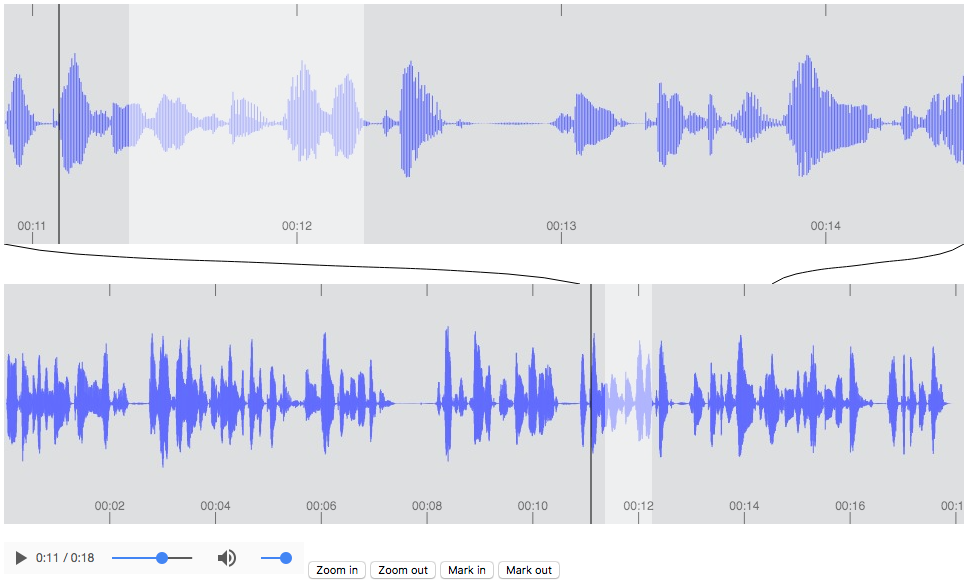
\includegraphics[width=\textwidth]{figs/beatmap.png}
  \caption{Example user interface that uses the BeatMap library.}
  \label{fig:beatmap}
\end{figure}

\subsection{Design}

We came across two challenges when designing BeatMap. Firstly, bitmap images of long audio files can be very large,
which makes it impractical for use over the web. Secondly, audio visualizations need to be able to zoom horizontally so
that users can view the visualization at different scales and levels of detail.

\paragraph{Tiling}
To bypass the problem of large image files, we designed BeatMap to use tiled bitmap images. This breaks the audio
visualization into many individual chunks, so that only the portion of the image currently being viewed needs to be
downloaded. Initial testing found that when playing, tiles were not being loaded in time, so we added a pre-loading
function that predicts which tiles will be displayed next and downloads them in advance.

\paragraph{Zoom}
We added a horizontal zoom function to allow audio visualizations to be viewed at different scales. We achieved this by
using multiple images, one for each scale, and allowing the user to switch between them. In addition to changing zoom
level within the main display, we added support for a linked secondary display that can view the same audio
visualization at a different zoom level (see Figure~\ref{fig:beatmap}). This enables users to simultaneously view the
entire audio recording at once, while also being able to see the visualization of the current playback position in
greater detail.

